\section{Satellite galaxies around a massive central}
The exercise is done in the script \lstinputlisting{satellite.py}. The necessary explanations of the methods used are in the comments of the code.
For question (a), the normalization factor A we obtain is the following: \lstinputlisting{normalization.txt}.
For question (b), we generate 3D satellite positions that statistically follow the satellite profile $n(x)$. We sample them from the probability density function $p(x)$, using the inverse transform sampling. We compare the distribution of the sampled points with $N(x)$, the analytical function describing the number of galaxies in a shell of thickness $dx$ at a given distance $x$. From Fig.\ref{fig:n_vs_hist}, we can see that the sampled points match the expected distribution. Nevertheless, we can see how the samples are not present in the first interval of $x$ values. Inverse sampling works by transforming uniform random numbers into samples from the desired distribution, using the cumulative distribution function (CDF) of the PDF. The CDF maps values from the sample space to the interval [0, 1], and its inverse can be used to map values from [0, 1] back to the sample space. In the case of smaller values, a small range of uniform random numbers can map to a large range of small values in the sample space, leading to undersampling in these regions.
This might explain why there is a discrepancy at smaller values in our histogram.

\begin{figure}[h!]
  \centering
  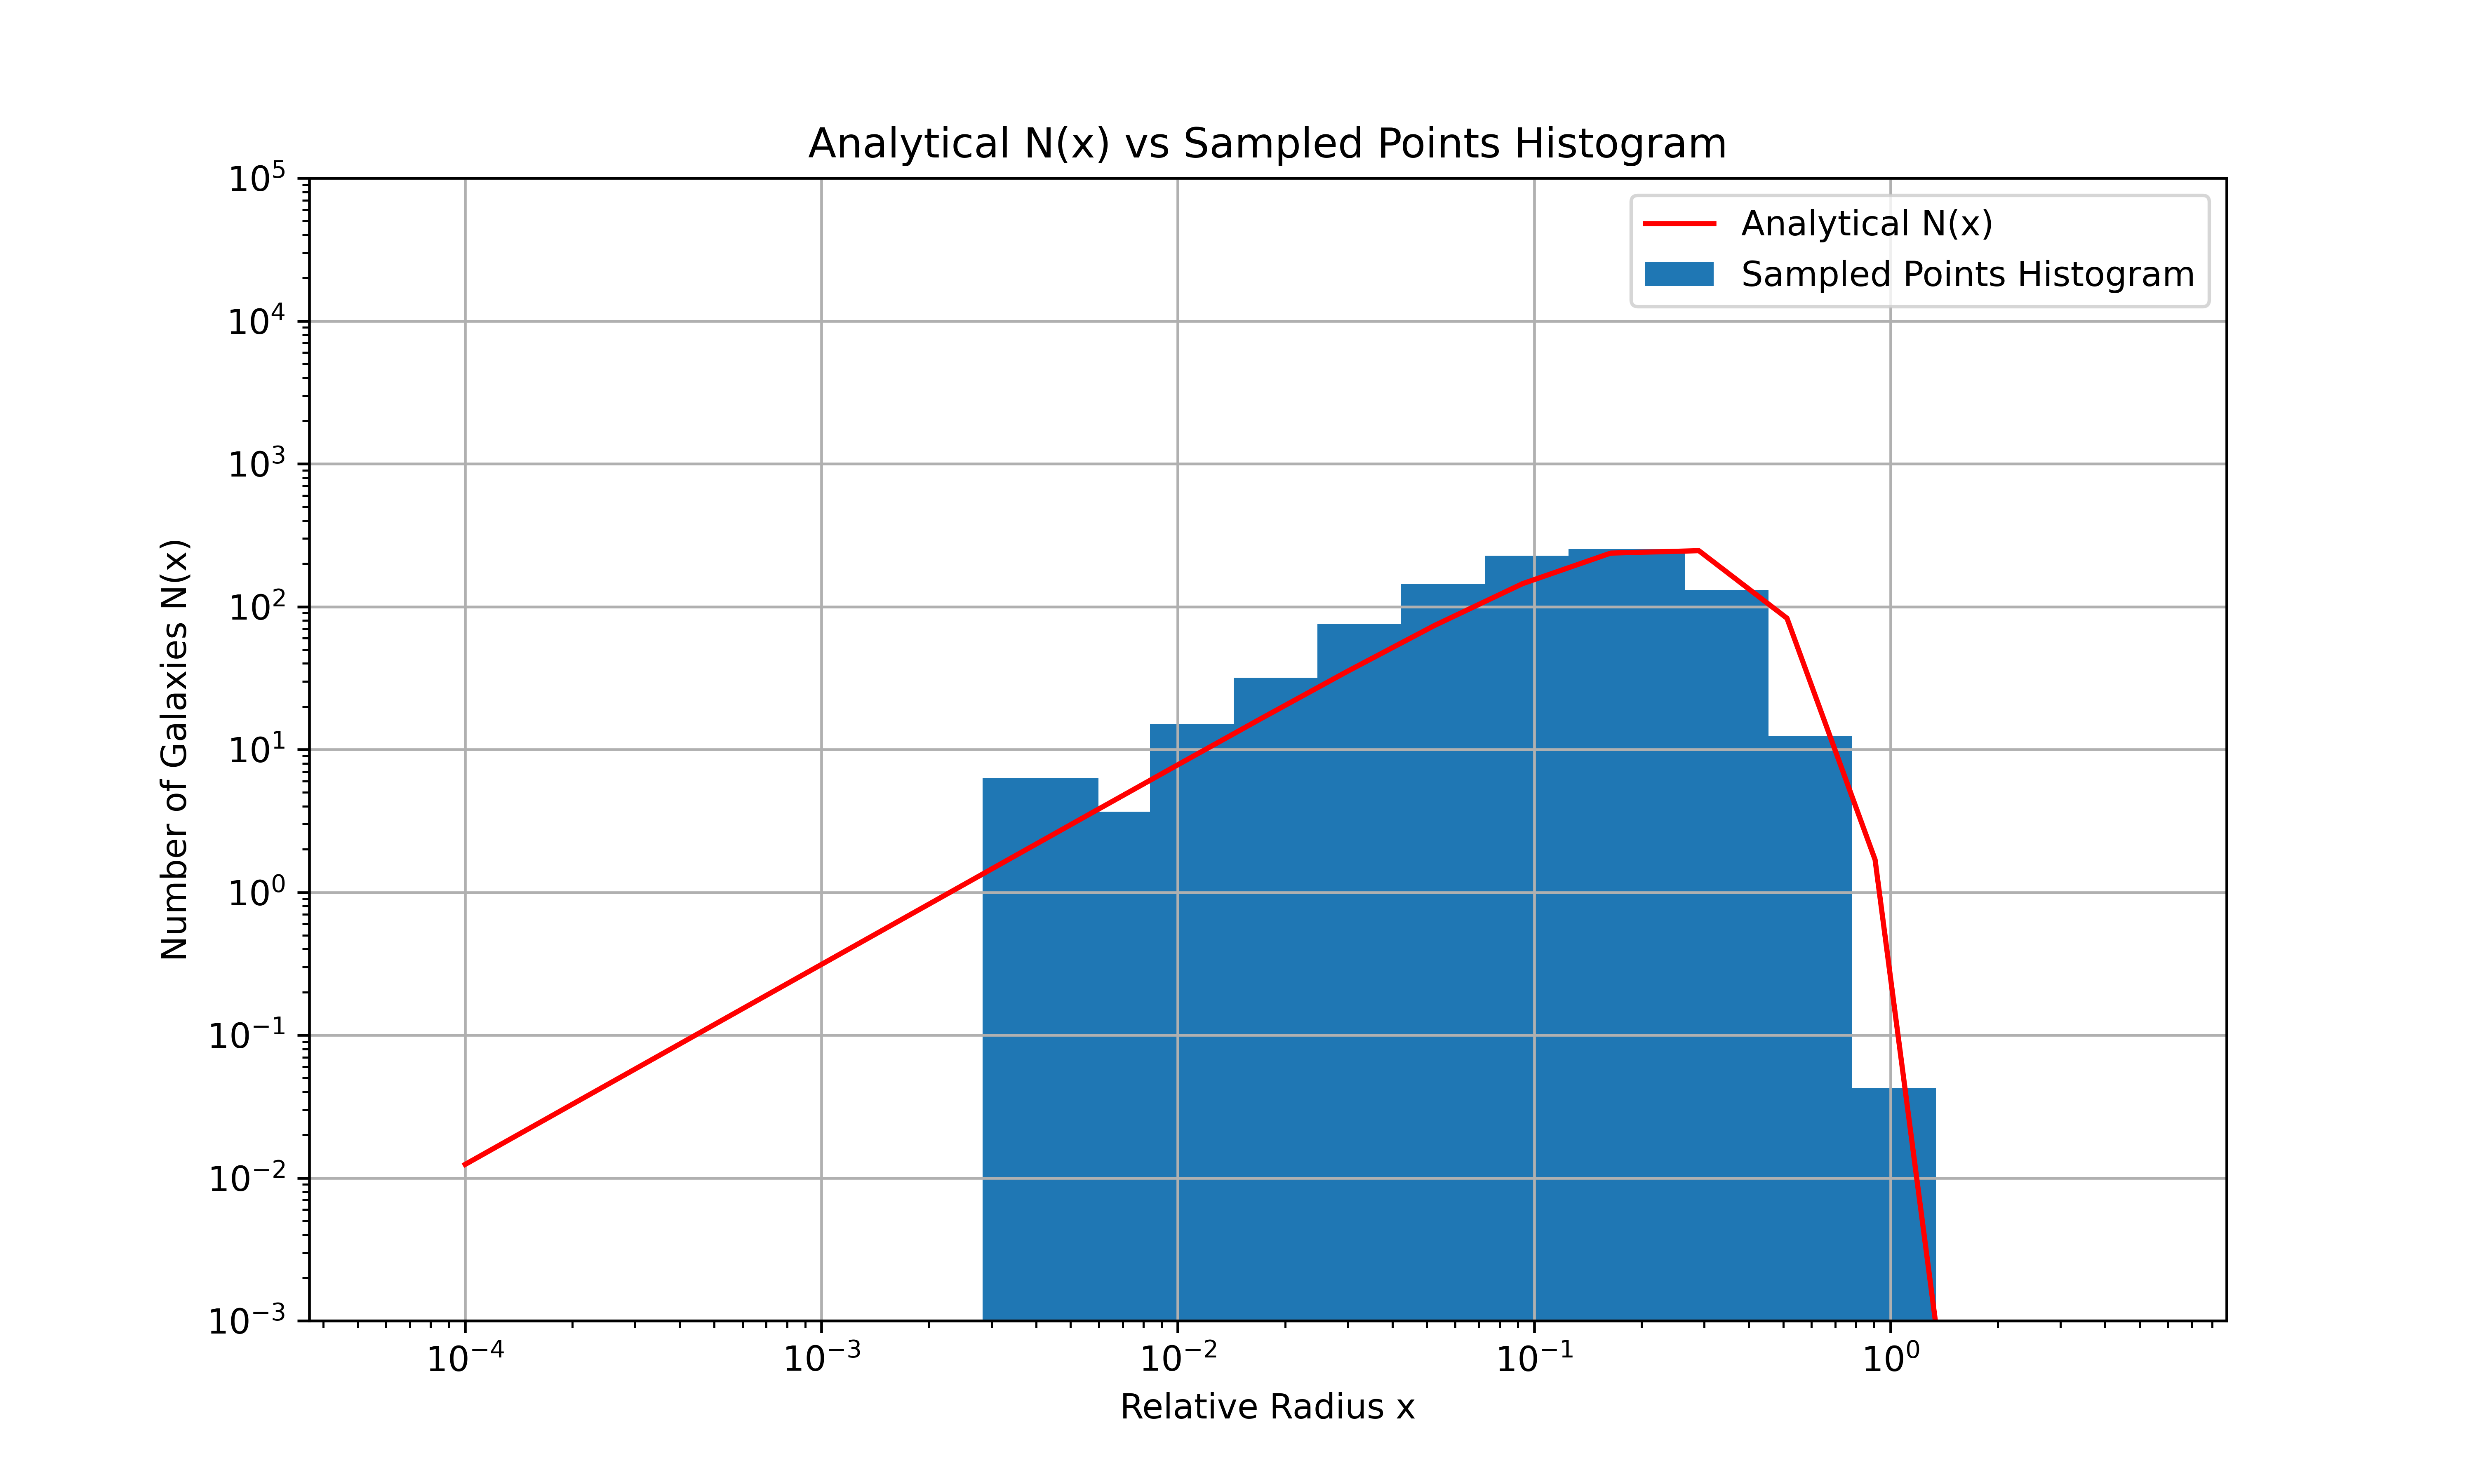
\includegraphics[width=0.9\linewidth]{./plots/my_solution_1b.png}
  \caption{Plot in logarithmic scale showing $N(x)$, function of the number of galaxies at given distance $x$, and the histogram of the 10000 sampled points. The sampled points match the analytical distribution, but there is a problem of undersampling in the region of smaller radii.}
  \label{fig:n_vs_hist}
\end{figure}

For question (c), we select 100 random galaxies using Reservoir sampling. It is an algorithm that chooses a random sample, without replacement, of k items from a population of unknown size n in a single pass over the items. 


\section{Heating and cooling in HII regions}

\begin{figure}[h!]
  \centering
  \includegraphics[width=0.9\linewidth]{./plots/my_vandermonde_sol_2b.png}
  \caption{Upper panel: Interpolation on a set of given data points via Neville's algorithm. The polynomial obtained fits the data points well in the range considered, in the same way the interpolation of LU decomposition does. Bottom panel: Absolute difference between the given points $y_i$ and our result $y(x)$, i.e. $|y(x) - y_{i}|$. The errors of Neville's algorithm reach very small values with respect to LU decomposition's ones. }
  \label{fig:neville}
\end{figure}

\begin{figure}[h!]
  \centering
  \includegraphics[width=0.8\linewidth]{./plots/my_vandermonde_sol_2c.png}
  \caption{Upper panel: Interpolation on a set of given data points via LU decomposition, with iterative improvement of the found solution (done with 1 and 10 iterations). Both the fits are going through all the data points exactly, hence the overlap. Bottom panel: Absolute difference between the given points $y_i$ and our result $y(x)$, i.e. $|y(x) - y_{i}|$. The trend is similar for the two implementations, with a small decrease in values reached by LU with 10 iterations.}
  \label{fig:lu_iter}
\end{figure}
